		\section{Overview}\label{reqoverview}
			\emph{Pawned} is a system for playing \index{6.170 Antichess} \emph{6.170 Antichess}, a variant
			of chess in which the goal 
			is to either lose all of your pieces (except the king) or checkmate your opponent. Antichess is 
			played between two opponents by moving pieces on a square board. The board is composed of 64 
			squares. The eight vertical lines of squares are called \emph{columns} and the eight horizontal 
			lines of squares are called \emph{rows}. The squares are colored black and white alternately as 
			seen in Figure \ref{standardchessboard}.
										
										\begin{figure}
											\begin{center}
												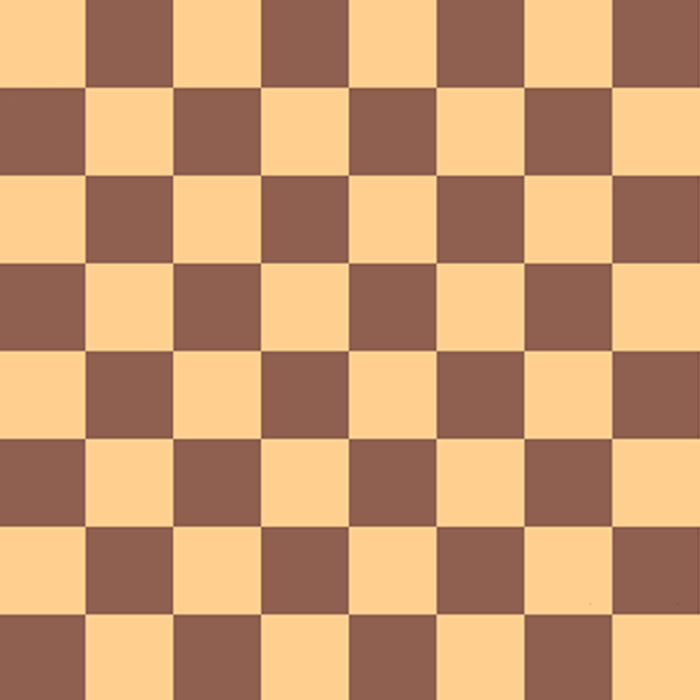
\includegraphics[width=150pt]{img/chessboard.png}
												\caption{A standard board for playing Antichess} 
												\label{standardchessboard}
											\end{center}
										\end{figure}

										The following document assumes familiarity with the rules of \emph{6.170 Antichess}. For a complete 
										description of the \emph{6.170 Antichess} rules, refer to Appendix \ref{6170acrules}. 
										%From this point
										%onward, the document uses the form \emph{Pawned does} when referring to the form \emph{Pawned should do}. 
										
										\emph{Pawned} is playable as a standalone application. Its basic mode of game is to have a human play 
										against a machine player using a Graphical User Interface (GUI). Additionally, \emph{Pawned} provides
										a standard interface to engage in multiplayer tournaments with other \emph{6.170 Antichess} players. 
										For a complete specification of this interface, refer to Appendix \ref{machineplayerspec}.
										
										\emph{Pawned}'s computer player does not simply make arbitrary moves, but rather bases them on
										decision heuristics that enable to play competitively, using multicore computing capabilities, when
										available. 
										
									 The \index{interface!Graphical User Interface} GUI has the following characteristics:
									 \begin{itemize}
									 	\item It contains:
										 \begin{itemize}
										 	\item A graphical representation of the current state of the board
										 	\item The name and color corresponding to each of the players
										 	\item The player that should move the piece next
										 	\item The remaining time on each player's clock
										 \end{itemize}	 			
										\item It allows:
											\begin{itemize}
												\item Graphical input mechanism. That is, a way for the user to input their
														moves using a mouse pointer
												\item Move validation and real time board status update 
												\item Easy access to information about the last move executed 
												\item Initiation of a new game
												\item Storage and retrieval of games. For the full documentation of 
														  the format used by \emph{Pawned} to save games, please refer to 
														  Appendix \ref{xmlformat} 
												\item Termination of the current game 
											\end{itemize}																									 	
									 \end{itemize}

						Finally, \emph{Pawned} provides a \index{interface!Command Line Interface} Command Line Interface (CLI) as specified in Appendix \ref{textuispec}. 

		\section{Revised Specification}\label{revisedspec}

		
			\emph{Pawned} supports extensibility in several ways. For that reason, \emph{Pawned} should be seen as a 
			\emph{Game Execution Environment} \index{Game Execution Environment}, and not merely a 
			\emph{6.170 Antichess Player}. The latter is just one game that is runnable within \emph{Pawned}.
			
				\subsection{Game Execution Environment}
						\emph{Pawned} allows the execution of a board game: a sequential activity between two players 
						who can manipulate pieces in an $n$-dimensional board according to a fixed set of rules. At any 
						given point, the game has one of two states: either running or terminated. This termation can occur
						 as a result of several conditions and may  be of different types. For example, in \emph{6.170 Antichess}, 
						 an example of a termination could come from a player being checkmated. Additionally, the game has a set of 
						 messages. These messages indicate game-specific information about the current state of a game. This 
						 information can vary from, for example, a message indicating that a current game of \emph{Chess} is 
						 in check, or any other relevant game information 
								
						A game can have observers. An observer can see the game dynamics while they happen but cannot participate 
						(i.e. cannot manipulate pieces in the board). A player can be thought of as an obsesrver who has the 
						additional faculty of manipulating pieces.
																			
						A game can be timed by a pair of timers, which limits the amount of time each player has throughout the 
						game. If a player runs out of time, the player loses the game.
								
				\subsection{6.170 Antichess}
						\index{6.170 Antichess}
						\emph{6.170 Antichess} is an example of a game that can be run in the Game Execution Environment. It 
						consists of two variants: \emph{Standard 6.170 Antichess}, and an extended edition of it, 
						\emph{6.170 Antichess with Encastle}, which is similar to the standard version, with additional 
						support for \emph{en passant} and \emph{castling} moves within the game. A complete analysis 
						of the rules and distinctions between both versions of \emph{6.170 Antichess} is included  
						in Section \ref{reqoverview} and detailed in Appendix \ref{6170acrules}. 
						 
						The players for \emph{6.170 Antichess} can be either two human players using the same 
						interface, one human player using a playing interface against a computer player, or two computer players
						being observed by a playing interface.
																			 
						\subsubsection{Playing Interface}
							\emph{Pawned} allows the users to play antichess in a \index{interface!Graphical User Interface} Graphical User 
							Interface (GUI) that shows the board and pieces. The revised GUI looks like that on Figure
							\ref{gui}. It consists of a main panel, a toolbar, four menu bars, and a status bar. The main panel 
							displays the following information:
								\begin{itemize}
									\item A graphical representation of the board and pieces. A numbering appears next to the board,
												allowing the user to easily reference a cell in the board.
									\item The name of the players along with the color of the pieces they are using.
									\item A timer for each player that shows how much time left a player has to complete all its moves.
												If no time limit is selected, the timers are not displayed.
									\item A move history displaying all the moves that have been made througout the game. The moves
												are displayed in extended chess notation format.
									\item The pieces each player has captured.
								\end{itemize}
							The main panel resembles that on Figure \ref{guimain}.
								
								%%% Complete GUI figure
								\begin{figure}
									\begin{center}
										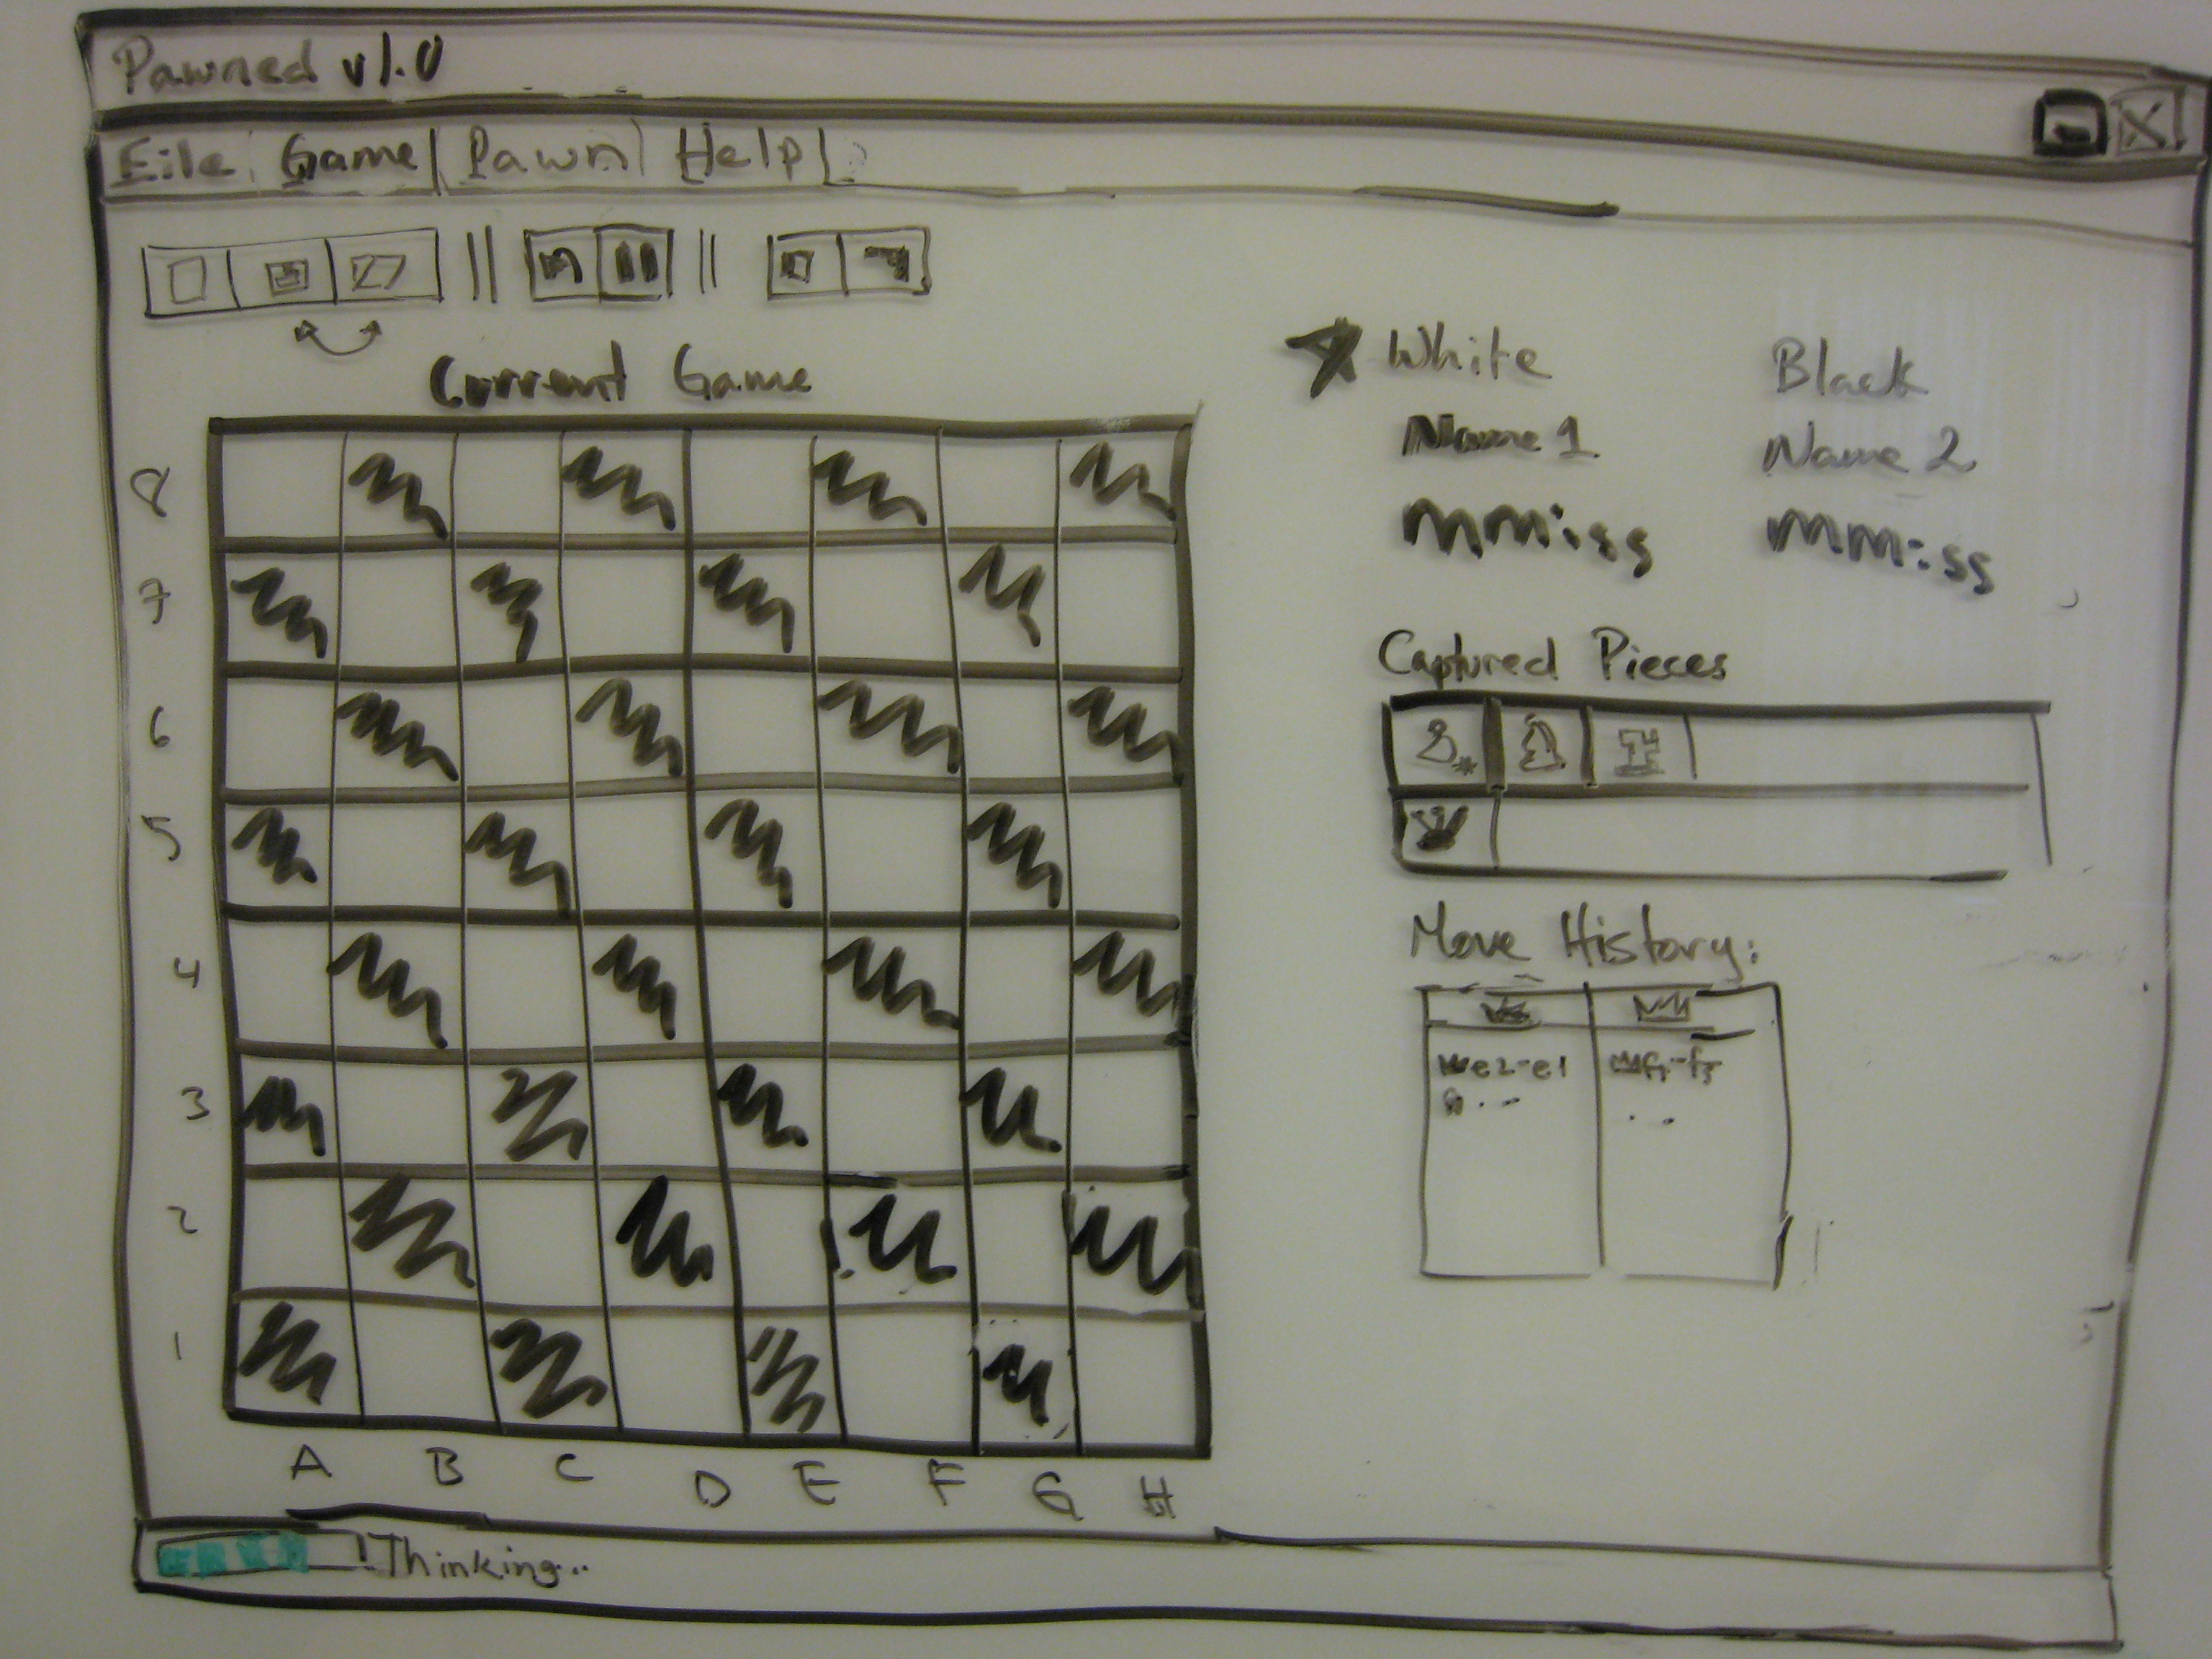
\includegraphics[width=220pt]{img/gui-sketch-main.jpg}
										\caption{\emph{Pawned}'s Graphical User Interface}
										\label{gui}
									\end{center}
								\end{figure}
								
								%%% GUI Main panel figure
								\begin{figure}
									\begin{center}
										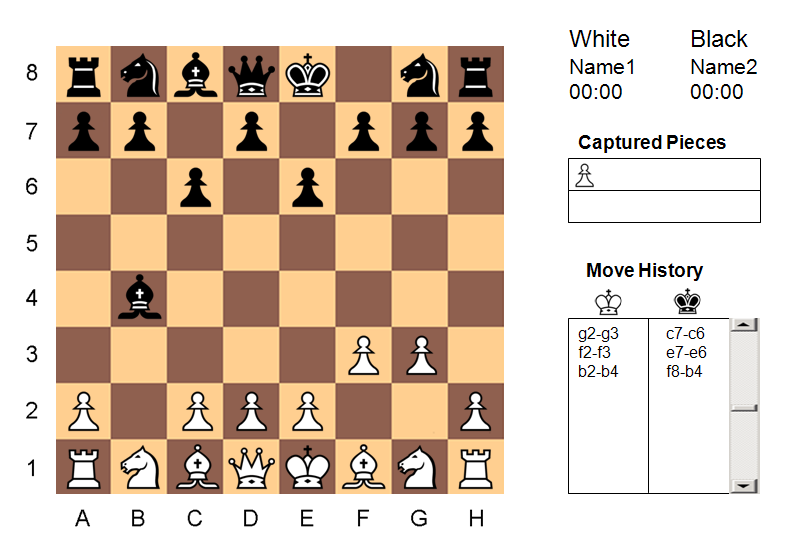
\includegraphics[width=220pt]{img/guiExample.png}
										\caption{\emph{Pawned}'s GUI Main Panel}
										\label{guimain}
									\end{center}
								\end{figure}
								
							The GUI indicates which player has the turn to play by highlighting his name, color and timer (if playing 
							with time limit). The possible moves a piece can perform are highlighted when a user puts the pointer on it.
							
							The four menu bars have the the following menu items (menu items with ``?'' are still under consideration):
								\begin{description}
									\item[File] New Game, Save Game, Load Game, Quit
									\item[Game] End game
									\item[Help] User's Manual, About...
								\end{description}
								
							The \textbf{New Game} option opens a window resembling that on Figure \ref{newgame} where the user has to 
							select the properties of the new 
							game. This window lets the user enter the names of the players, and select if each player is Human or 
							Computer. If the Computer player is chosen, the user can select the intelligence level of the player, from
							among several options. The user also has to select between a game with ``Unlimited Time'', or enter the 
							desired time limit for each player. Finally, there is an option to select the type of game (i.e. 
							\emph{Standard 6.170 Antichess}, \emph{6.170 Antichess with Encastle}, etc).
							
								%%% GUI New game window
								\begin{figure}
									\begin{center}
										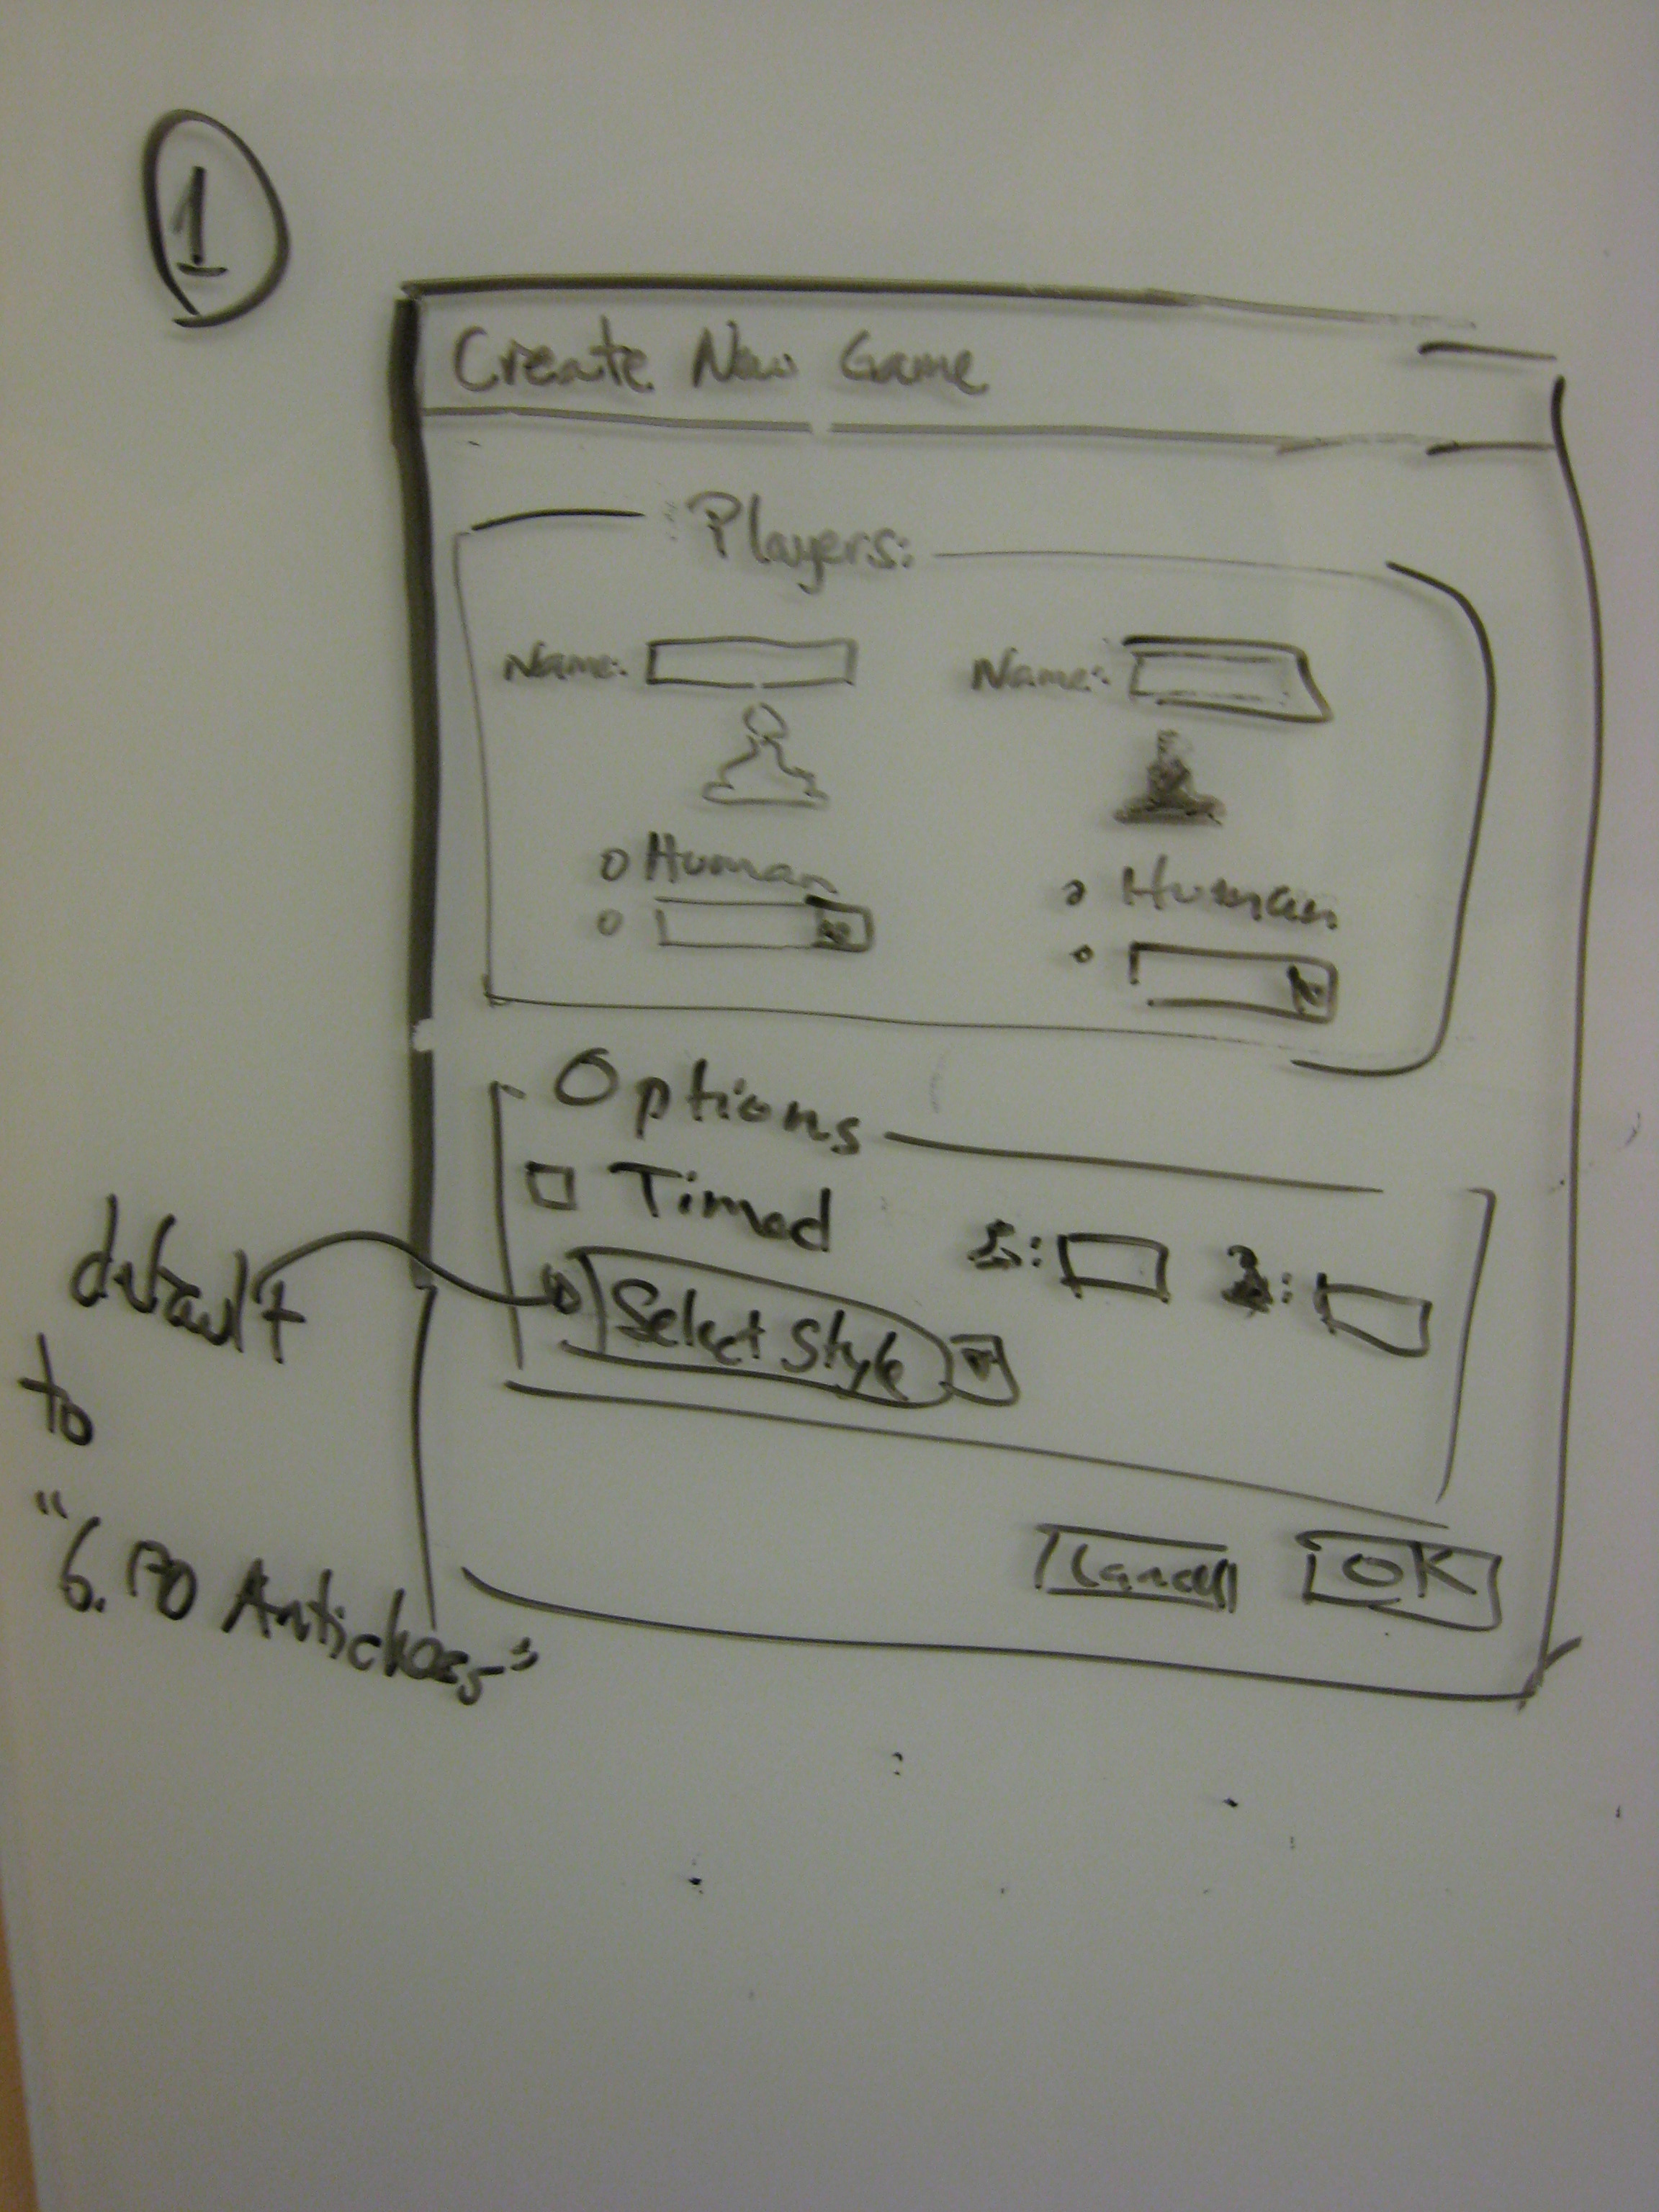
\includegraphics[width=220pt]{img/gui-sketch-menu-new.jpg}
										\caption{\emph{Pawned}'s New Game Window}
										\label{newgame}
									\end{center}
								\end{figure}
							
							The \textbf{Save Game} option opens a file chooser window that lets the user select where the game
							file is going to be saved.
							
							The \textbf{Load Game} option prompts a window similar to that of \emph{New Game}. The user is able to
							select the players that will resume the game, as well as select a route to a valid 
							\emph{Pawned} game file. After selecting a game to load, the user has to select the players that will
							resume the game.
							
							The \textbf{Quit} option exits \emph{Pawned}.

							The \textbf{End game} option allows the user to end a game without exiting the application.
							
%							The \textbf{Display Options} option lets the user select between different graphical options, 
%							such as different piece images, and different boards.
							
							The \textbf{User's Manual} option opens \emph{Pawned} users' manual.

							Finally, the \textbf{About...} option shows information about the \emph{cool} creators of \emph{Pawned}.

							
							The operation mechanisms for the Command Line Interface (CLI) to enable the user to select their preferred 
							game variant when a new game is started are detailed in Appendix  \ref{textuispec}. 
							
							
%			Talk about the extensibility of \emph{Pawned}, including that the game board is not restricted to an 8x8 square 
%			board, but can be any n-dimensional board, supports several rulesets,
			
%			Pause the game.
			
%			(extended XML format)
			
%			Move history - better ply language (capture shit and check, checkmate)

		\section{Performance}
			\emph{Pawned}'s \emph{6.170 Antichess} AI player makes use of parallel computing. This player running
			on a multicore processor beats the same AI player running on a single core processor at least 51\% of the time.  

		\section{Problem Analysis}\label{problem-analysis}

			\subsection{Execution Environment}
			In order to fulfill the requirements outlined above, \emph{Pawned} defines an abstract \index{player} 
			\textbf{player} that can provide a \emph{ply} upon request. A \index{ply} ply is a set of actions, such as 
			moving or adding a piece to the board, that constitutes	a player's move for its turn. For example, in regular 
			chess, castling is a ply that consists of two moves.
			
			These players are able to interact with a \index{controller} \textbf{controller}, who is in charge of finalizing 
			a ply, and executing it. The controller is also in charge of notifying the appropriate player	that it is its turn 
			to play, and notifying the players if a termination condition has been met or if a player has run out of time, in 
			which case this player would effectively lose. Additionally, the controller is responsible for creating, loading,
			and saving games. The controller can be thought of a referee that mediates communication between the players and 
			the game itself.
			
			Finally, the last component is the actual \index{game} \textbf{game model}, which holds all the relevant information about the 
			game. This includes the status of the game board, the history of the plies, and the \emph{rule set} being	used. 
			The rule set contains the set of global rules (i.e. the set of rules that govern the movements of any piece) along 
			with the types of pieces supported and how each piece can locally move. The game model can then validate any move 
			and determine whether there is a winner by using the rule set.
			
			A rule set \index{rule set} for a game consists of five parts: 
			\begin{itemize}
				\item A set of \index{rule set!global rules} \emph{global rules} that govern the movement of all the pieces in the 			
							game. 
							For example, a global rule in \emph{6.170 Antichess} is that if a player is in check, 
							then it \emph{must} perform a ply	that will put him out of check.
				\item A set of \index{rule set!local rules} \emph{local rules} that specify the valid plies of a set of 
							supported pieces.
							For example, a local rule in \emph{6.170 Antichess} is that a bishop can move diagonally 
							to an empty cell or one that contains a piece of another color, without jumping any pieces.
				\item A set of \index{rule set!termination conditions} \emph{termination conditions} that specify whether a game 
							has been 
							finished. This termination could be a result of a game having a winner, a game resulting in a draw, or
							other termination. 
							For example, a termination condition in \emph{6.170 Antichess} is checkmate.  
				\item A set of \index{rule set!messages} \emph{game messages} that reflect events in the game. `Check' is an example
							of one of such messages in \emph{6.170 Antichess}.
				\item A \index{rule set!turn management} \emph{turn management} mechanism to determine the next turn, i.e. the 
							rules governing who should play after a move
						  has been executed by a given player. For example, in \emph{6.170 Antichess}, the players should play 
						  in an alternated fashion, except if a player is in stalemate.
				\item A set of \emph{supported boards and plies} for the particular game specified by the rule set. 
							The rule set possesses information about the initial board configuration for the game. 
							For example \emph{chess board} would be the supported board for \emph{6.170 Antichess}, 
							with the initial board configuration as specified by Appendix \ref{6170acrules}. 
			\end{itemize}
      See	Figure \ref{componentdiagram} for a visual depiction of these components. The \emph{Factories} component 
      refers to the set of all possible plies and boards supported for a given rule set.  
			
				\begin{figure}
					\begin{center}
						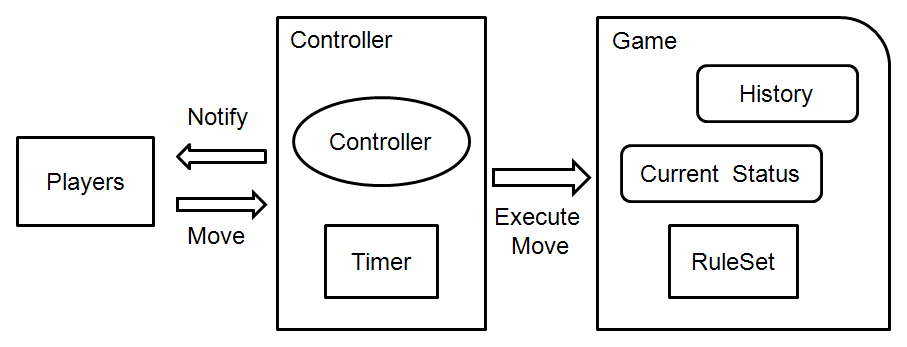
\includegraphics[width=220pt]{img/componentDiagram.png}
						\caption{Component diagram}
						\label{componentdiagram}
					\end{center}
				\end{figure}
			
					
			
			\subsection{Considerations}  %How-to's
				\subsubsection{Handling plies}
					Even though all the players have access to the board's status at any given point in time, any player that wishes
					to perform a ply must do so through the controller. This will ensure that the board does not get changed when it
					should not. If an artificial intelligence (AI) player wants to simulate plies on a board to choose its next ply, 
					then it must do so on copies of the board.
					
					The controller notifies each player when a ply has been executed. 

				\subsubsection{Controlling the game}
					When the controller decides that it is someone's turn, it notifies the player that a ply should be provided. 
					The controller will then wait for this player to submit a valid ply, prompting it again in case the player
					submitted an invalid ply. 
					
					Once the player submits a valid ply, the controller notifies the model and delegates the turn to the 
					appropriate player. In the case that the move just executed results in a termination state (e.g.
					in the case that a player has been checkmated in \emph{6.170 Antichess}), 
					the controller's behavior is specified by Section \ref{winner}. 
					
					
	%			2. mention that we need to compute just after a move has been executed. Obtaining the moves (Piece + ruleset)
	%			(why in ruleset instead of game? cuz AIplayer needs access to it). 

	%				How to check when someone wins (RuleSet) or loses (RuleSet + Timer)

				\subsubsection{Determining a finishing condition}\label{winner}
				  A game finishes when a termination condition has been met, including the possibility that 
				  a player has run out of time. 
				  In the case of \emph{6.170 Antichess}, these conditions are checkmate, win by depletion of pieces, or
				  double-sided stalemate, as specified by Appendix \ref{6170acrules}. 
			%%restart here	  
				  When one such event has occured, the game notifies the controller immediately after the terminating ply has been 
				  executed. The controller then notifies each of the players of the termination condition.
				  The controller notifies the players and observers when the time for the current player has been 
				  depleted. These in turn act in the way that they deem appropriate (e.g. a GUI might display the termination 				   					information, or an AI player might stop computing successive moves, if any).

					Since the game model is in charge of holding the status of the game, it will always contain the information 
					regarding whether the game is running or if it has terminated, along with its termination condition. 

				\subsubsection{Ply validity}
					As was stated before, the rule set for a game consists of five parts. Given a rule set, a ply is valid if it
					satisfies all the rules (unless a global rule overrides a local rule, in which case compliance with the global rule 
					deems the ply valid).
	 
						\begin{description}
							\item[Local Rules\index{rule set!local rules}] These specify the valid plies of a set of supported pieces. They 										are piece-specific. A piece has knowledge of its valid plies given its location on a board.
							\item[Global Rules\index{rule set!global rules}] Given the union of all the local rules for all pieces, 
																											the global rules add or remove valid plies. 
						\end{description}

					Since the controller needs to check a ply for validity before executing it, and the players might want to 
					view the valid moves frequently (for example a GUI determining all the valid pieces for display to 
					the user), \emph{Pawned} provides this validation in constant time. 
			
			\subsection{Architecture} %implementation of how-to's
				\emph{Pawned}'s game execution environment uses the following abstract modules. See Figure \ref{conceptualDiagram}
				for a visual depiction of these modules.
				
					\begin{description}
						\item[Piece] A Piece represents a game piece, whose state and behavior depends on a RuleSet and a Board.
												 A Piece can contain information about its color (black or white), type, initial position as 
												 defined by the RuleSet, as well as other information it finds necessary.

												 A Piece can be created in two ways. In both ways a color for the Piece must be specified. If 
												 a Board is also given, then the new Piece will add itself to the Board at a default initial 
												 position (defined by the RuleSet). If all the possible initial positions are occupied, an 
												 invalid position message is returned to the invoker. If a Board is not specified, then the 
												 Piece is created but it is not contained in any Board. It can subsequently be added to a Board 
												 at a specified cell position.

												 A Piece can provide information about its color, type, and the Plies it can perform (given a
												 Board). These Plies are only those which conform with the local rules specified in the 
												 RuleSet. Notice that \emph{all} the knowledge about a valid Ply must lie within the Piece itself; the 
												 Board will not assume anything except that no two Pieces can occupy the same cell. In this 
												 sense, a Piece has to have the information of whether it can capture a Piece of its own color 
												 or not (allowing addition of Pieces such as the AntiKing).

												 Notice that some rules might force the Pieces to be able to determine information about other 
												 Pieces in a Board. For example, the rule of castling in Chess requires a King to determine 
												 whether a Rook has been moved during the game. To accomplish this, a Piece has a mechanism 
												 that allows it to receive a notification every time a Ply has been executed in the Board. It 
												 can then retrieve what it needs to update the information it cares about. In some cases no 
												 information is really needed, such as for a Bishop, but this functionality allows \emph{Pawned} 
												 to easily support any Plies that involve this type of information.

												 This poses another problem: each Piece now holds important information that needs to be 
												 recovered when a game is loaded. Thus, \emph{Pawned} is able to load a game that was saved 
												 by reproducing the information by executing all the Plies specified in its move history. 
												 A deeper discussion of the alternative mechanisms for holding state information and 
												 the ruleset - piece interaction can be found in Section \ref{board-discussion}. 
												
						\item[Board] A Board provides the representation of the gaming board. It consists of a set of cells that 
												 may contain at most one Piece. The cells are referenced via a group of $n$ indices. In this 
												 sense, a Board represents an $n$-dimensional board. \emph{6.170 Antichess} uses a Board where
												 $n=2$.

												 A Board serves simply as a cell structure that contains Pieces. It makes the follwing assumptions:
												 	\begin{itemize}
												 		\item No two Pieces can occupy the same cell.
												 		\item A Piece cannot occupy two cells at the same time.
												 		\item When a Ply is executed, a Piece occupying the ending cell of the Ply will be 
												 					captured and removed from the Board.
												 	\end{itemize}
												 	However, it does not assume anything about the Pieces it contains or about the game that is 
												 	being played.
												 	
												 	It can determine the position of a given Piece, get all the Pieces of a given 
												 	color that are currently in the Board, execute a Ply and notify the Pieces that are currently 
												 	in the Board, and clone itself. When executing a Ply, it returns a set of captured Pieces.
												 	
												 	Pieces can also be added and removed from a Board outside the context of a game. This allows 
												 	for Boards to be arbitrarily set in any fashion.

						\item[Move] A Move represents a transition from one cell to another within a Board. In other words, a move 
												contains information about the starting and ending cell positions in a Board. A Move can be 
												created by specifying a starting cell position and an ending cell position.
						
						\item[Ply] A Ply represents a sequence of actions, that can be either Moves, Removal or Additions. A Move 
											 is defined previously. A Removal is an action by which a piece previously present in a board is no 														 longer registered as contained by the board. An Addition is an action by which a piece not 
											 previously present in a board is registered as contained by the board.
						
						\item[Game] A Game constitutes the central mechanism for game control. It contains information about the game 
												rules using a RuleSet. Additionally, it contains a Board representing the current configuration
												along with captured pieces and ply history, a set of possible Plies and the current Turn, State, 
												and Messages. 
												
												As previously specified, States can either be active or terminated (along with its Termination
												condition), and Messages can be any type of condition that is occuring in the game, 
												such as the \emph{check} condition, in \emph{Standard Chess}. 

												A Game can be created from an initial Board configuration, along with a RuleSet for the 
												specified game. 
												
												A Game provides 
												\begin{itemize} 
													\item Information on whether a given Ply would be valid considering the current configuration 
																and turn. Because this mechanism is assumed to be used often, it should be as efficient 
																as possible.
													\item A mechanism that informs the caller about the current Board, Turn, State, and Messages 
																upon request.
													\item A mechanism for providing the game history (a sequence of Plies in the order they were 
																executed since the beginning of the game).
													\item A mechanism for retrieving captured pieces for each of the players. 
													\item A mechanism for executing a given Ply and provides information of who should play next.
																It should also notify the invoker if the Ply resulted in a termination condition.
												\end{itemize}
												
						\item[Controller] A Controller is the mediator between the Players, Observers and Game. It holds information 
															about the Timer, as well as the Players and Observers currently engaged in the game. 
														  
														A Controller can be created by providing the two Players, a RuleSet, and a Board. The Boad will be
														setup using the list of pieces supported by the game, as provided by the RuleSet. Since each piece
														knows where to place itself, this process should be unambiguous. 
														
														  A Controller provides
														  \begin{itemize}
														  	\item An asynchronous messaging system for the suscribed Players and Observers for notification
														  				regarding addition of Messages, States, Terminations, and Time Depletion. 
																\item A messaging system for notifying the subscribed Players about their turn
																\item A system for managing observers in the observer list 
																\item A game saver 
														  	\item A Controller Factory for creating controllers from previously saved games
														  	\item Execute moves on the game 
														  \end{itemize}  
												
					
						\item[Observer] An Observer is the most basic subscriber to a controller. It should contain 
													  a mechanism for subscribing to the Controller's messaging system on notifications. 
													  
						\item[Player] A Player is a type of Observer. He should also provide a mechanism for receiving messages from the
													turn delegation system provided by Controller. 
					\end{description}
				
				\begin{figure}
					\begin{center}
						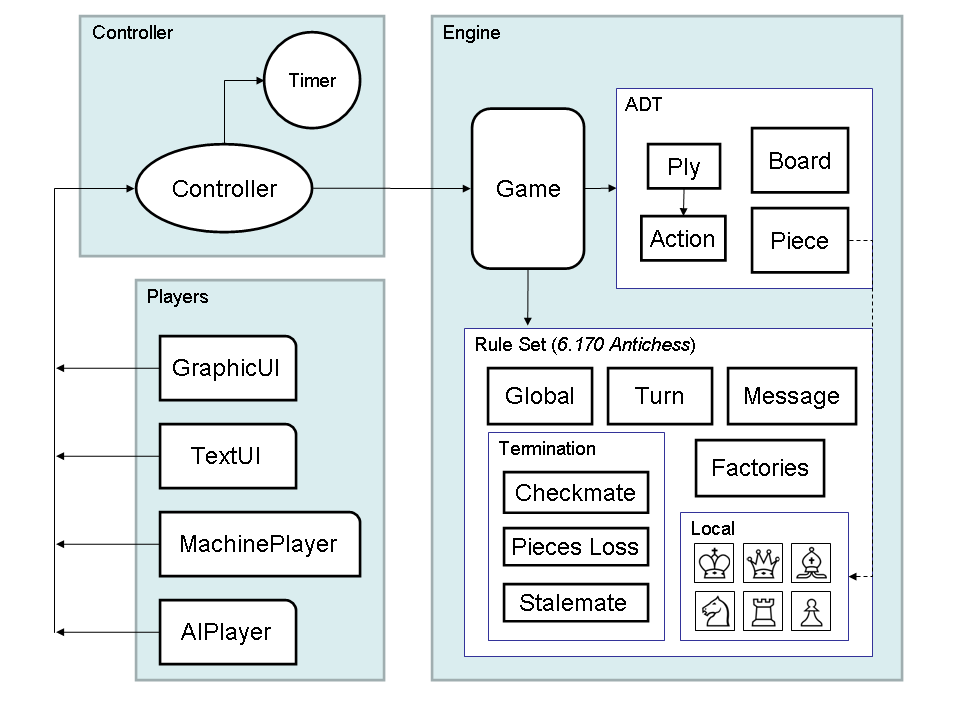
\includegraphics[width=250pt]{img/conceptualDiagram.png}
						\caption{Conceptual diagram}
						\label{conceptualDiagram}
					\end{center}
				\end{figure}
			
% We need to talk about standard antichess here. 

%				Talk about \emph{Pawned} in terms of interfaces and what they do.
%				Then explain how the architecture address issues outlined above.
				
%				Do we need a separate class for Move? Yes
%
%				Do we need a separate class for Cell? No
%
%				The implementation will use a separate instance of a Piece to represent each
%				piece in the game, instead of using an interning pattern. Pawns need to know if
%				they have moved already or not, and to queen. Can this be handled by the RuleSet
%				though? It would be better because then its easier and less computationally
%				intensive to clone a Board.
%
%				Who has permission to modify the board? Controller or Game -> Game
%
%				Should Board keep a list with captured pieces? No
%
%				How to refer to a cell in a Board? With an N length array of integers
%				
%			\subsection{Extensibility}
%				As stated previously, \emph{Pawned} is extensible in a number of ways. The previous high-level outline brings
%				forward several issues with regard to the extensibility of \emph{Pawned}. These are discussed in detail in this
%				section.
%				
%				First and foremost, \emph{Pawned} is not restricted to gameplay on a standard 8x8 square board. Any board whose
%				cells can be addressed by a sequence of numbers $a_1, a_2, \ldots, a_n$ is a valid board. Thus,
%				the board is
%				
%				Talk about what could be extended in \emph{Pawned}. That is, talk about what a Rule Set must provide, what a Board 
%				should be...
%				
%				
%			
%				Timers
%				
%				How to separate piece behavior from the board as much as possible (defining �usability� of a cell)
%				
%				Piece: notice that how a piece moves depends on a board and ruleset. Example: two
%				rectangular boards with different cell ordering. Why do we care? To make the
%				program extensible.
%
%				possibility of weird moves.
%				Since we use more information than the XML, we have to recreate the game for games that do not contain our
%				additional XML extensions. Otherwsie we can rebuild the pieces and then fast - build the board by serialization.
%				
%				new piece motion, turns (not only 1-1, but m-n).